\documentclass{article}

% PACKAGES
\usepackage[margin=0.75in]{geometry}
\usepackage{amsmath}
\usepackage{amssymb}
\usepackage{graphicx}
\usepackage{subcaption}
\usepackage{hyperref}
\usepackage{wrapfig}
\usepackage{float}
\usepackage{enumitem}

\title{ECE 269 - Final Project\\Orthogonal Matching Pursuit}
\author{Eric Weise}
\date{December 17, 2020}

\begin{document}

\maketitle

This project is hosted on GitHub:
\url{https://github.com/ericdweise/ece269/blob/master/report.pdf}




\section{Background}



Orthogonal Matching Pursuit (OMP) is a greedy algorithm that can be used to recover sparse signals 
There is a dearth of literature summarizing the usage and limits of OMP for sparse signal recovery.
The purpose of this work is to provide and implementation and analysis of OMP.
First effectiveness of singal recovery is evaluated in section 3.
Then, in sections 4 and 5 the effectiveness of OMP is evaluated on signals with added noise.
Finally, in section 6, OMP signal recovery is applied to compressive sampling in images both with and without noise added.



\section{The OMP Algorithm}
The OMP algorithm is described here.
Given a signal $x \in \mathbb{R}^N$ the following steps are taken to recover the signal:

First a random Gausian matrix is created, $A \in \mathbb{R}^{M \times N}$, where $M<<N$.

The columns of $A$ are normalized.

Calculate $y = Ax$

The first residual is calculated: $r_0 = y$

The support set is initialized as empty: $\Lambda_0 = \{\}$

{\bf Main loop:}
\hspace{15px}
\begin{enumerate}[leftmargin=2cm,labelsep=0cm,align=left]
    \item Find the column of A with maximum correlation to residual: $\lambda_k = arg\;max_j |\langle a_j, r \rangle|$
    \item Update the support set: $\Lambda_k = \Lambda_{k-1} \cup \lambda_k$
    \item Find the recovered signal $\hat{x}_k$, which is the Least Squares solution to $A_{\Lambda_k}\hat{x}_k = y$
    \item Update the residual: $r_{k+1} = y - \Lambda_k \hat{x}_k$
\end{enumerate}


This loop will continue until one of two conditions is met:
\begin{enumerate}[leftmargin=1.5cm,labelsep=0cm,align=left]
    \item Given a threshold we can stop when $||r||_2$ is less than this threshold.
    \item Provided that the sparsity level, $s$, of $x$ is known, we can stop after the loop executes $s$ times.
\end{enumerate}

The recovered signal is $\hat{x}_k$, where $k$ is the final iteration count of the main loop.


\subsection*{Error Analysis}
Given a signal $x$ and its recovered analog $\hat{x}$, the normalized error is calculated as:
\begin{align*}
    \frac{||x-\hat{x}||_2}{||x||_2}
\end{align*}


\subsection*{Implementation}
The implementation of the OMP used in this project can be found here:

\url{https://github.com/ericdweise/ece269/blob/4e869d18719761ae3458ef0244da7af4768095fc/tools.py#L148}








%%%%%%%%%%%%%%%%%%
%%%   PART C   %%%
%%%%%%%%%%%%%%%%%%

\newpage

\section{Noiseless Signal Recovery ({\it part c})}


The Exact Signal Recovery (ESR) rate is very highly correlated to s, and somewhat correlated to M.
This is evident in the sharp increase in the Probability of ESR for low s.
For all matrix sizes the probability of ESR is zero for a sparsity level above $\frac{N}{10}$,
but this threshold decreases slightly as the height of the matrix, $M$ decreases.

The Normalized Error plots show roughtly the inverse trend as that in the ESR plots:
The Error rate is low for small sparsity, and reach a plateau close to 1.2.

\begin{figure}[H]
    \captionsetup{width=.75\linewidth}
    \centering
        \includegraphics[width=0.25\textwidth]{plots/c-recov_N-20.png}
        \includegraphics[width=0.25\textwidth]{plots/c-recov_N-50.png}
        \includegraphics[width=0.25\textwidth]{plots/c-recov_N-100.png}
        \newline
        \includegraphics[width=0.25\textwidth]{plots/c-error_N-20.png}
        \includegraphics[width=0.25\textwidth]{plots/c-error_N-50.png}
        \includegraphics[width=0.25\textwidth]{plots/c-error_N-100.png}
        \caption{Noiseless support set recovery. Top row: The probability of Exact Support Recovery. Bottom row: Normalized error of recovered signal. NOTE: The ESR and the error plots are viewed from different angles.}
\end{figure}















%%%%%%%%%%%%%%%%%%%
%%%   PART D1   %%%
%%%%%%%%%%%%%%%%%%%

\newpage
\section{Noisy Signal Recovery With Known Sparsity ({\it Part d-i})}

In this experiment the same procedure was applied in the noiseless signal recovery, but two major differences were made:
\begin{enumerate}
    \item After the original sparse signal $x$ is generated, random noise is added to every element in $x$.
        This resulting noisy vector, $x_{noise}$ is used to calculate $y = Ax_{noise}$
    \item The OMP loop is terminated after $s$ iterations, where $s$ is the sparsity level of $x$.
\end{enumerate}
Two experiments are performed.
The first experiment adds noise drawn from a normal distribution with mean 0 and variance 0.05.
The second experiment adds noise drawn from a normal distribution with mean 0 and variance 1.

It should be noted that the Normalized error was calculated using the original signal, not the noisy signal.

As we might predict, adding small amounts of noise changes the ESR and Normalized Error plots slightly, while adding more noise significantly degrades the probability of ESR.
For a noise variance of 0.05 the ESR and Normalized error plots are almost identical to the noiseless case.
However, for a noise variance of 1 the probability of ESR decreases significantly, and never rises above 75\%.
The normalized errors in the variance 1 case are also significancly higher, never dropping lower than 0.5, and plateauing at 1.4, an increase of about 15\% over noiseless recovery.


\begin{figure}[H]
    \captionsetup{width=.75\linewidth}
    \centering
        \includegraphics[width=0.25\textwidth]{plots/d1-recov_N-20_noise-0.05.png}
        \includegraphics[width=0.25\textwidth]{plots/d1-recov_N-50_noise-0.05.png}
        \includegraphics[width=0.25\textwidth]{plots/d1-recov_N-100_noise-0.05.png}
        \newline
        \includegraphics[width=0.25\textwidth]{plots/d1-error_N-20_noise-0.05.png}
        \includegraphics[width=0.25\textwidth]{plots/d1-error_N-50_noise-0.05.png}
        \includegraphics[width=0.25\textwidth]{plots/d1-error_N-100_noise-0.05.png}
        \caption{Noisy support set recovery {\bf variance=0.05}. Stop condition achieved when loop count is the sparsity of the input signal. Top row: The probability of Exact Support Recovery. Bottom row: Normalized error of recovered signal. NOTE: The ESR and the error plots are viewed from different angles.}
\end{figure}


\begin{figure}[H]
    \captionsetup{width=.75\linewidth}
    \centering
        \includegraphics[width=0.25\textwidth]{plots/d1-recov_N-20_noise-1.png}
        \includegraphics[width=0.25\textwidth]{plots/d1-recov_N-50_noise-1.png}
        \includegraphics[width=0.25\textwidth]{plots/d1-recov_N-100_noise-1.png}
        \newline
        \includegraphics[width=0.25\textwidth]{plots/d1-error_N-20_noise-1.png}
        \includegraphics[width=0.25\textwidth]{plots/d1-error_N-50_noise-1.png}
        \includegraphics[width=0.25\textwidth]{plots/d1-error_N-100_noise-1.png}
        \caption{Noisy support set recovery {\bf variance=1}. Stop condition achieved when loop count is the sparsity of the input signal. Top row: The probability of Exact Support Recovery. Bottom row: Normalized error of recovered signal. NOTE: The ESR and the error plots are viewed from different angles.}
\end{figure}
















%%%%%%%%%%%%%%%%%%%
%%%   PART D2   %%%
%%%%%%%%%%%%%%%%%%%

\newpage
\section{Noisy Signal Recovery ({\it part d-ii})}

In this experiment the same procedure was applied in the previous section, except that the stop condition is changed:
\begin{enumerate}
    \item The OMP loop is terminated when the the two norm of the residual, $||r_k||_2$ is less than 0.001.
\end{enumerate}

Two experiments are performed.
The first experiment adds noise drawn from a normal distribution with mean 0 and variance 0.05.
The second experiment adds noise drawn from a normal distribution with mean 0 and variance 1.

It should be noted that the Normalized error was calculated using the original signal, not the noisy signal.

As might be expected, the results are similar identical to the previous section.
This stands to reason because if exact support recovery does not happen after $s$ iteration of the main loop, it will not happen after more iterations,
That is: the agreement between $x$ and $\hat{x}$ will not increase if the loop count exceeds the sparsity level of $s$.


\begin{figure}[H]
    \captionsetup{width=.75\linewidth}
    \centering
        \includegraphics[width=0.25\textwidth]{plots/d2-recov_N-20_noise-0.05.png}
        \includegraphics[width=0.25\textwidth]{plots/d2-recov_N-50_noise-0.05.png}
        \includegraphics[width=0.25\textwidth]{plots/d2-recov_N-100_noise-0.05.png}
        \newline
        \includegraphics[width=0.25\textwidth]{plots/d2-error_N-20_noise-0.05.png}
        \includegraphics[width=0.25\textwidth]{plots/d2-error_N-50_noise-0.05.png}
        \includegraphics[width=0.25\textwidth]{plots/d2-error_N-100_noise-0.05.png}
        \caption{Noisy support set recovery {\bf variance=0.05}. Stop condition achieved when the 2-norm of residual is less than 0.001. Top row: The probability of Exact Support Recovery. Bottom row: Normalized error of recovered signal. NOTE: The ESR and the error plots are viewed from different angles.}
\end{figure}


\begin{figure}[H]
    \captionsetup{width=.75\linewidth}
    \centering
        \includegraphics[width=0.25\textwidth]{plots/d2-recov_N-20_noise-1.png}
        \includegraphics[width=0.25\textwidth]{plots/d2-recov_N-50_noise-1.png}
        \includegraphics[width=0.25\textwidth]{plots/d2-recov_N-100_noise-1.png}
        \newline
        \includegraphics[width=0.25\textwidth]{plots/d2-error_N-20_noise-1.png}
        \includegraphics[width=0.25\textwidth]{plots/d2-error_N-50_noise-1.png}
        \includegraphics[width=0.25\textwidth]{plots/d2-error_N-100_noise-1.png}
        \caption{Noisy support set recovery {\bf variance=1}. Stop condition achieved when the 2-norm of residual is less than 0.001. Top row: The probability of Exact Support Recovery. Bottom row: Normalized error of recovered signal. NOTE: The ESR and the error plots are viewed from different angles.}
\end{figure}















%%%%%%%%%%%%%%%%%%%
%%%   PART D3   %%%
%%%%%%%%%%%%%%%%%%%

\newpage
\section{Image Recovery ({\it Part d-iii})}

\subsection*{Compressive Sampling and Signal Recovery Methods}

Compressive sensing is a rich field.
The goal is to take the fewest number of samples and maintain recoverability of the source signal.
First we must find an appropriate orthonormal basis ${\psi_1, \ldots, \psi_N}$.
A signal $x$ can be created as a linear combination of the elements $\psi_i$.
The sparse sensing happens in this basis, choosing the highest correlated components in this orthonormal basis to the original signal.
Recovery of the sparse signal, $x_s$, the sparse representation of $x$ in the $\Psi$ basis, can be performed using OMP.
In this paradigm, $\Psi$ is the matrix whose columns are the O.N. basis, ${\psi_1, \ldots, \psi_N}$,

The purpose of this experiment is to demonstrate the recoverability of a compressed image.
The image will be compressed using and recovered for different sparsity levels.

These are the steps used in Compressive Sensing and Signal Reconstruction:
\begin{enumerate}
    \item First, a random gaussian matrix matrix is made, $\Phi \in \mathbb{R}^{M \times 64}$.
    \item The image is broken into $8 \times 8$ subimages.
    \item The subimage is transformed into frequency space using a Discrete Cosine Transform.
        The $64 \times 64$ DCT matrix forms $\Psi$.
    \item The transformed $8 \times 8$ subimage is rearranged into a vector $x \in \mathbb{R}^{64}$
        The order uses the zig-zag pattern demonstrated in {\it figure 6} to bias low frequency coefficients in Fourier space.
    \item {\bf Compressive Sensing} The largest $s$ elements in $x$ are retained. The rest are set to zero. This sparse vector is denoted $x_s$
    \item Calculate $y = \Phi x_s$. ($y \in \mathbb{R}^M$)
    \item Perform OMP to recover $\hat{x} \in \mathbb{R}^{64}$.
        The stop condition is set to $||\Phi \hat{x} - y||_2 < 10^{-3}$
    \item $\hat{x}$ is rearranged to an $8 \times 8$ array using the zig-zag ordering.
    \item The Inverse Discrete Cosine Transform, $\Psi^{-1}$, is applied to convert the recovered subimage back to image space.
\end{enumerate}

In the above steps $y = \Phi \Psi x_s$ is the first residual used in OMP to reconstruct the signal, $x$.
This process is repeated for every $8 \times 8$ subimage.
For this experiment it was found that a Gaussian random matrix $\Phi$ with size $30 \times 64$ was both time performant and recovered images with good detail.

\begin{figure}[H]
    \captionsetup{width=.5\linewidth}
    \centering
        \includegraphics[width=0.5\textwidth]{assets/zigzag.jpg}
        \caption{The Zig-zag ordering. In the DCT Basis this preferences low frequency components over higher frequency components.}
\end{figure}


\subsection*{Error Measurements}

To measure the efficacy of the recovered image the Peak Signal to Noise Ratio (PSNR) is calculated.
PSNR is used on the entire, large image and its reconstructed analog, not to the $8 \times 8$ subimages.
The PSNR is calculated as:

\begin{align} 
    PSNR = 10 \cdot log_{10} \frac{MAX^2}{MSE}
\end{align}
where
\begin{align} 
    MSE = \frac{1}{mn} \sum_{i-0}^{m-1} \sum_{j-0}^{n-1} \Big[ I(i,j) - K(i,j) \Big]^2
\end{align}
is the mean squared error of the images, $I$ and $K$ are the original and recovered images, $m, n$ are the number of rows and columns in the images, and $MAX$ is the maximum possible value a pixel can have.


\newpage
\subsection*{Image Recovery After Compressive Sensing}

This experiment was performed on four images.
The imags were chosen to show a varying level of complexity.
The recovered images and some recovered images are shown in figures 7-10.

Even at a very low sparsity level there is significant image reconstruction.
At $s/N = 2/64$ we begin to see some texture, although finer details are not recovered.
However, even at low sparsity levels, around 8, we can see more details being recovered.
Notice the texture in the elephant's skin, the tree branches under the arch, and the hairs of the koala start to appear.

In figure 11 we can see the PSNR plotted as a function of sparsity in the measurement basis for each of the images.
In all but one of the images, the PSNR increases as the measurements become less sparse.
The complex images, elephant, koala, and arch, have lots of detail, which correspond to high frequency components in the DCT space.
However, the recovery tends to plateu between a sparsity level of 4 and 8.
This corresponds to a compression level between 6.25\% and 12.5\%.


Interestingly the spiral has peaks at a sparsity level of 3.
This is because the image has large regions where the pixels change very slowly in real space.
This means that they can be represented using very few vectors in the DCT basis.
Approxmation of these regions with higher frequency vectors will degrade the image in real space.

\begin{figure}[H]
    \captionsetup{width=.75\linewidth}
    \centering
        \includegraphics[width=0.25\textwidth]{images/arch.png}
        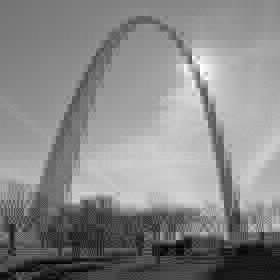
\includegraphics[width=0.25\textwidth]{images/arch-recovered_02.png}
        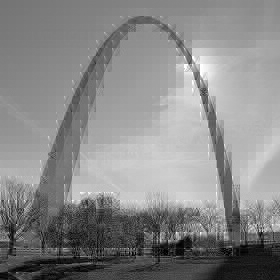
\includegraphics[width=0.25\textwidth]{images/arch-recovered_08.png}
        \caption{The original image of the arch (left) recovered image with s=2 (center) and recovered image with s=8 (right)}
\end{figure}

\begin{figure}[H]
    \captionsetup{width=.75\linewidth}
    \centering
        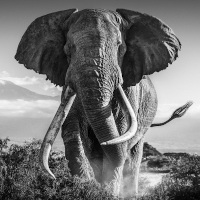
\includegraphics[width=0.25\textwidth]{images/elephant.png}
        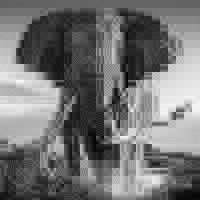
\includegraphics[width=0.25\textwidth]{images/elephant-recovered_02.png}
        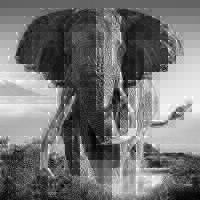
\includegraphics[width=0.25\textwidth]{images/elephant-recovered_08.png}
        \caption{The original image of elephant (left) recovered image with s=2 (center) and recovered image with s=8 (right)}
\end{figure}

\begin{figure}[H]
    \captionsetup{width=.75\linewidth}
    \centering
        \includegraphics[width=0.25\textwidth]{images/koala.png}
        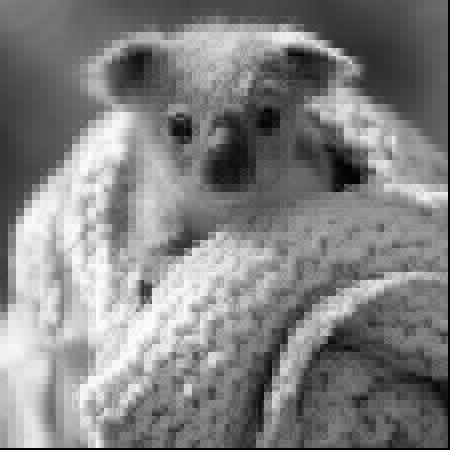
\includegraphics[width=0.25\textwidth]{images/koala-recovered_02.png}
        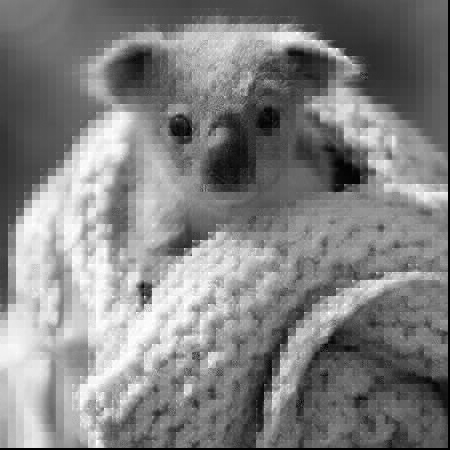
\includegraphics[width=0.25\textwidth]{images/koala-recovered_08.png}
        \caption{The original image of the koala (left) recovered image with s=2 (center) and recovered image with s=8 (right)}
\end{figure}

\begin{figure}[H]
    \captionsetup{width=.75\linewidth}
    \centering
        
\includegraphics[width=0.25\textwidth]{images/spiral.png}
        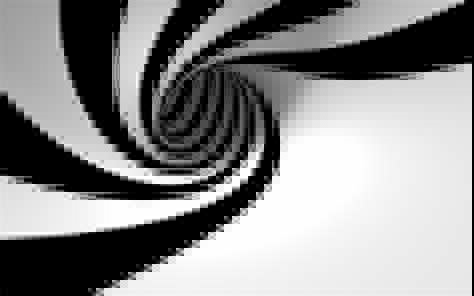
\includegraphics[width=0.25\textwidth]{images/spiral-recovered_02.png}
        
\includegraphics[width=0.25\textwidth]{images/spiral-recovered_08.png}
        \caption{The original image of the spiral (left) recovered image with s=2 (center) and recovered image with s=8 (right)}
\end{figure}



\begin{figure}[H]
    \captionsetup{width=.5\linewidth}
    \centering
        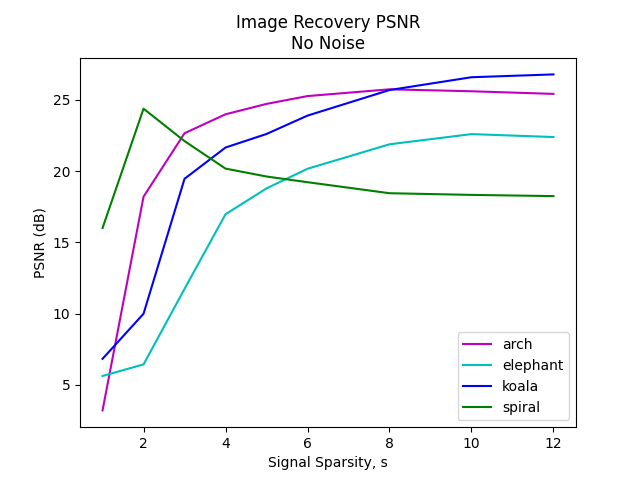
\includegraphics[width=0.5\textwidth]{plots/d3-no-noise.png}
        \caption{PSNR measured for varying sparsity levels and for different levels of added noise.}
\end{figure}




\newpage
\subsection*{Image Recovery With Added Noise}

The process of reconstructing the noisy image is the same as the previous section.
Before the process of compressive sensing begins , however, random noise is added to the image.
Each pixel has added a random number drawn from a normal distribution.
This is done twice, first with a variance of 10, then again with a variance of 50.
The mean for both experiments is zero.
Since the images have a bit depth of $2^8$, a variance of 10 has a noise level of approximately $2.5\%$,
and a variance of 50 has a noise level of approximately $25\%$.

The error measurements are also the same as noiseless image recovery.
It should be noted that the PSNR is calculated using the clean original image.
That is, the image with no added noise.


Figures 12 and 13 show the result of reconstructing the noisy koala image for the two noise levels.
It is evident, especially in figure 13, that the recovered image is less noisy for more sparse measurements.
When using a sparsity level of 2 in the measurement basis stores more information from the original image than a sparsity level of 8.
This is again evident in figure 14, which plots the PSNR vs sparsity level for the different noise levels.
This is because the recovery biases lower frequency coefficients in the DCT domain, which selects out the high frequency Gaussian noise.
However, at a certain sparsity level the PSNR starts to decrease as the reconstructed image starts to include the high frequency noise.


\begin{figure}[H]
    \captionsetup{width=.75\linewidth}
    \centering
        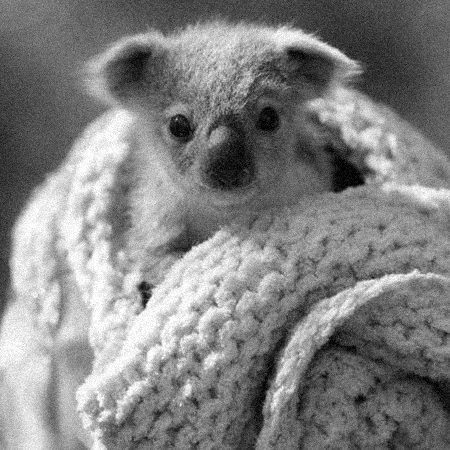
\includegraphics[width=0.25\textwidth]{images/koala_noise-10.png}
        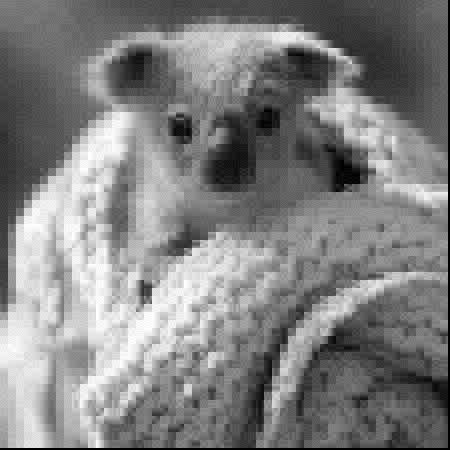
\includegraphics[width=0.25\textwidth]{images/koala_noise-10-recovered_02.png}
        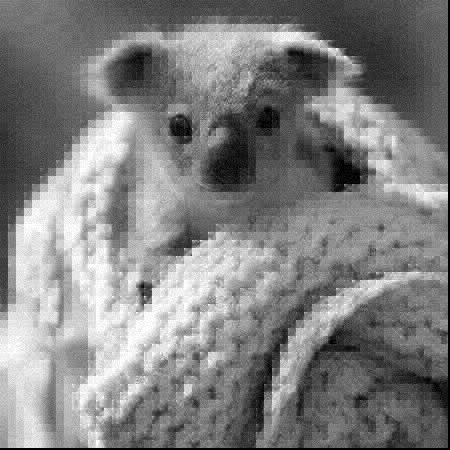
\includegraphics[width=0.25\textwidth]{images/koala_noise-10-recovered_08.png}
        \caption{Results for image reconstruction with added noise {\bf variance=10}. From left to right: Image with added noise. Recovery with sparsity 2. Recovery with sparsity 8.}
\end{figure}


\begin{figure}[H]
    \captionsetup{width=.75\linewidth}
    \centering
        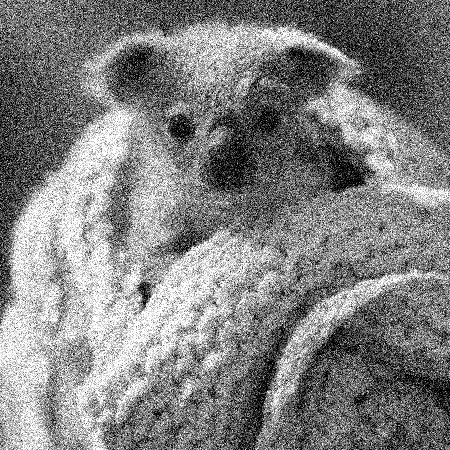
\includegraphics[width=0.25\textwidth]{images/koala_noise-50.png}
        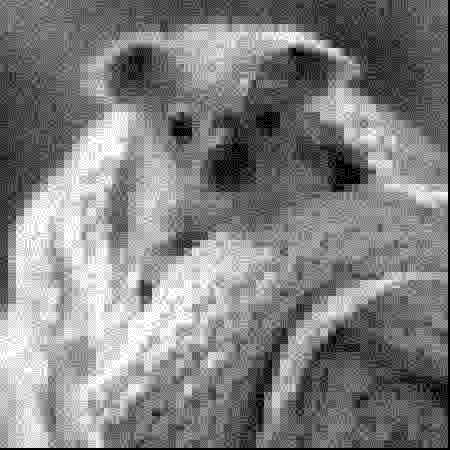
\includegraphics[width=0.25\textwidth]{images/koala_noise-50-recovered_02.png}
        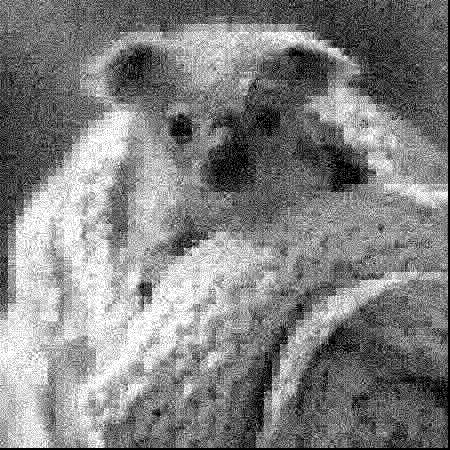
\includegraphics[width=0.25\textwidth]{images/koala_noise-50-recovered_08.png}
        \caption{Results for image reconstruction with added noise {\bf variance=50}. From left to right: Image with added noise. Recovery with sparsity 2. Recovery with sparsity 8.}
\end{figure}


\begin{figure}[H]
    \captionsetup{width=.9\linewidth}
    \centering
        \includegraphics[width=0.45\textwidth]{plots/d3-noise-10.png}
        \includegraphics[width=0.45\textwidth]{plots/d3-noise-50.png}
        \caption{Peak Signal to Noise Ratio as a function of sparsity for noisy images. Left noise variance=10, right noise variance=50.}
\end{figure}

\end{document}
